\documentclass{article}


\usepackage{PRIMEarxiv}

\usepackage[utf8]{inputenc} % allow utf-8 input
\usepackage[T1]{fontenc}    % use 8-bit T1 fonts
\usepackage{hyperref}       % hyperlinks
\usepackage{url}            % simple URL typesetting
\usepackage{booktabs}       % professional-quality tables
\usepackage{amsfonts}       % blackboard math symbols
\usepackage{nicefrac}       % compact symbols for 1/2, etc.
\usepackage{microtype}      % microtypography
\usepackage{fancyhdr}       % header
\usepackage{graphicx}       % graphics
\graphicspath{{media/}}     % figures live under media/

\usepackage{amsmath,amssymb}
\usepackage{algorithm}
\usepackage{algpseudocode}

\raggedbottom

%Header
\pagestyle{fancy}
\thispagestyle{empty}
\fancyhead[LO]{Integrating Traditional and Deep Learning Methods to Detect Tree Crowns in Satellite Images}

%% Title
\title{Integrating Traditional and Deep Learning Methods to Detect Tree Crowns in Satellite Images}

\author{
  Ozan Durgut* \\
  Software \& Design Group \\
  Analog Devices \\
  Istanbul, Türkiye\\
  \texttt{ozan.durgut@analog.com} \\
   \And
  Beril Kallfelz-Sirmacek* \\
  School of Arts and Sciences \\
  University of Mary \\
  Bismarck, ND, USA\\
  \texttt{berilkallfelz@gmail.com} \\
  \And
  Cem Ünsalan*\\
  Faculty of Engineering \\
  Yeditepe University \\
  Istanbul, Türkiye\\
  \texttt{unsalan@yeditepe.edu.tr} \\
}


\begin{document}
\maketitle


\begin{abstract}
Global warming, loss of biodiversity, and air pollution are among the most significant problems facing Earth, and monitoring forests is central to addressing them. Automatic tree crown detection from satellite imagery is therefore an important task, approached by both traditional image-processing and deep-learning methods. In this study we ask a specific question: once a strong ensemble of deep detectors has been applied, is there anything a traditional method can still contribute? We combine five deep detectors with weighted boxes fusion (WBF) and a traditional pipeline (illumination-invariant color and a Gabor filter bank feeding a watershed/local-maxima detector) through a rule-based integration step. Evaluating on a benchmark of 222 test images containing 13{,}552 trees under one-to-one matching, we report precision, recall, and $F_1$ for every method rather than recall alone. Our central finding is that the traditional step recovers 448 true crowns (3.3 percentage points) that lie \emph{beyond the detection ceiling of the full six-model deep-learning stack at its most permissive thresholds} --- trees no detector proposes at any confidence. We show these recovered crowns are systematically small (a median crown area $2.44\times$ below detected crowns) and spectrally faint, which explains why appearance-trained detectors miss them and a texture/local-maxima operator recovers them. A lightweight appearance gate on the traditional-only detections removes the non-tree false positives they introduce, so the integrated detector dominates the WBF ensemble on the precision--recall frontier ($F_1$ 0.921 $\rightarrow$ 0.924 at a recovery-preserving operating point). Finally, we show on an independent benchmark from a different biome and sensor (US airborne NEON forests, using the field-standard DeepForest detector) that the same mechanism replicates: the recovered crowns are again the small ones ($1.91\times$ smaller). We report the advantages, the precision cost, and the limitations of the approach.
\end{abstract}


\keywords{Tree crown detection \and Feature extraction \and Joint probability map \and Deep learning \and Weighted boxes fusion \and Segmentation \and Detector complementarity}
\let\thefootnote\relax\footnotetext{*These authors contributed equally to this work.}



\section{Introduction}\label{sect:intro}

Forests and terrestrial plants produce $28\%$ of Earth's oxygen, making trees vital for sustainability \cite{GFRA}. Uncontrolled destruction of trees is one of the main causes of recent global issues such as global warming, air pollution, desertification, and intensified natural disasters \cite{forest_climate_change, forest_carbon_emission}. Human activities, including agriculture, livestock grazing, and urban expansion, are the primary causes, leading to continuous forest decline over the past 30 years. Despite the legal attempts, only 18\% of forests are currently under protection \cite{GFRA, brazilian_law, turkey_law_1, turkey_law_2}. Monitoring methods like LiDAR scanning, drone-based analysis, and sampling are used but have limitations and are unsustainable. On the other hand, correctly inventorying trees requires knowing their exact location and calculating their canopy area. Tree density provides insights into forest health and carbon storage capacity, while canopy widths reflect photosynthesis potential. Therefore, it is crucial to detect tree crowns. Traditional and deep learning based methods applied to satellite imagery can provide an efficient solution.

Recent studies demonstrate that traditional and deep learning methods for tree crown detection are often used separately. Traditional methods, such as template matching and local maxima-based techniques, have shown notable success in tree detection \cite{Korpela20032006, huo2020individual}. However, these methods can run into problems, particularly for studies focused on identifying small tree crowns, as the limited detail in crowns can impede accurate detection \cite{Korpela20032006}. Furthermore, Larsen~\emph{et al.}~\cite{larsen2011comparison} revealed that tree detection algorithms based on traditional methods alone are insufficient when using images from different regions. Deep learning based object detection methods are highly effective in tree detection. In our previous study, we analyzed swin transformers, RCNN, YOLO, and DETR, for tree detection and observed their strengths \cite{durgut2025multi}. Other studies support these findings; for instance, Xiao~\emph{et al.}~\cite{xiao2023csswin} improved tree detection performance by combining swin transformers with U-Net, and Ren~\emph{et al.}~\cite{ren2024local} modified swin transformers to make semantic segmentation of trees more successful.

Despite the individual success of traditional and deep learning based approaches, studies combining their results remain scarce in literature. Although Niccolai~\emph{et al.}~\cite{niccolai2010decision} did not explicitly combine these methods, their rule-based algorithm utilized local neighborhood analysis. Hybrid methods that integrate traditional segmentation techniques with U-net like CNNs demonstrate improved accuracy and show the complementary strengths of both approaches \cite{korznikov2021using, moussaid2021tree}. However, these works assert complementarity qualitatively; to our knowledge, no prior study \emph{quantifies}, on a labeled benchmark, how many trees a traditional operator recovers beyond a strong deep-learning ensemble, nor characterizes \emph{which} trees those are.

The objective in this study is to enhance tree crown detection by leveraging the strengths of traditional and deep learning based detection approaches within a rule-based integration, and --- crucially --- to measure and explain the complementarity between the two. In our previous work, we integrated five deep learning methods using weighted boxes fusion (WBF) \cite{durgut2025multi}. Here we extract additional information by applying traditional methods, combine the two through a rule-based procedure, and evaluate the result rigorously with precision, recall, $F_1$, and mean average precision under one-to-one matching.

\paragraph{Contributions.} We make the following contributions, and are explicit about the novelty of each:
\begin{itemize}
  \item \textbf{(Primary)} A quantified, benchmark-backed measurement of the \emph{complementarity} between traditional and deep detectors for tree crowns: a traditional operator recovers 3.3\% of trees beyond the full six-model deep-ensemble ceiling, and we characterize \emph{why} --- the recovered crowns are systematically small and spectrally faint. Prior hybrid studies assert complementarity; we measure and explain it.
  \item \textbf{(Generalization)} We replicate the mechanism on an independent benchmark from a different biome and sensor (US airborne NEON forests) using the field-standard DeepForest detector: the recovered crowns are again the small ones.
  \item \textbf{(Methodological)} A rule-based integration procedure that decides, per candidate, whether to trust the detector, a neighbor, or the traditional evidence; and a lightweight appearance gate that removes the false positives the traditional step introduces, yielding a tunable recovery/precision operating curve.
  \item \textbf{(Evaluation)} A rigorous re-evaluation protocol (one-to-one matching with precision/recall/$F_1$ and COCO mAP, plus a precision--recall operating-curve analysis) that corrects the recall-only scoring common in this sub-area.
\end{itemize}

\section{Traditional Methods for Tree Crown Detection}

Traditional methods are useful for object detection in satellite images, particularly when computational power and labeled data are limited. They can complement deep learning algorithms, improving true positives and reducing false negatives. We provide the corresponding workflow in Fig.~\ref{fig:workflow_traditional} and discuss each step below.

\begin{figure*}[htbp]
\centering
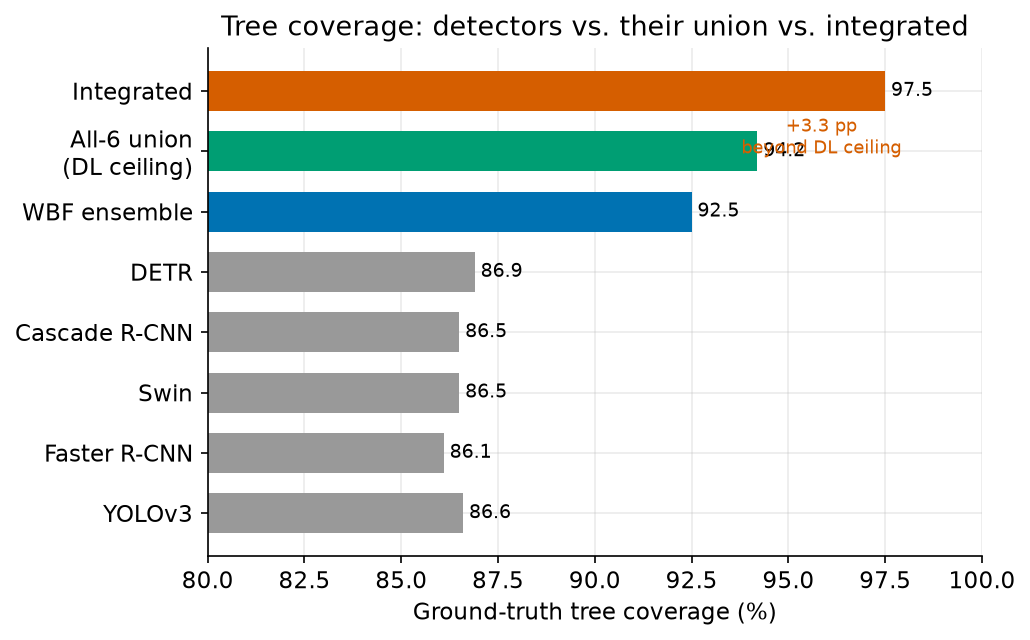
\includegraphics[width=1\textwidth]{fig_coverage_ladder.png}
\caption{Ground-truth tree coverage by each detector, the union of all six detectors at their most permissive thresholds (the deep-learning detection ceiling), and the integrated method. The integrated method reaches trees beyond the ceiling of the entire deep-learning stack.}\label{fig:workflow_traditional}
\end{figure*}

\subsection{Feature Extraction}

We calculate a feature value for each pixel and use these values in later steps to select pixels that carry the characteristics of a tree crown. We extract two features: an illumination-invariant color feature and a Gabor texture feature.

\subsubsection{Illumination-invariant Color}

To extract vegetation color robustly, we work in a normalized-rgb (chromaticity) space, in which each channel is divided by the per-pixel intensity sum. This representation is invariant to overall brightness and shading, which is essential given the strong sun/shadow variation in satellite imagery. On these chromaticity coordinates we compute an excess-green index, $2g - r - b$, as the color evidence for a tree crown. Unlike a fixed threshold in HSV space, this feature does not depend on absolute brightness and therefore survives illumination changes across a scene.

\subsubsection{Gabor Filter Bank}

Our second feature provides information about local texture. Following the systematic filter-selection scheme of Jain and Farrokhnia~\cite{JAIN19911167}, each channel is filtered with a bank of Gabor filters spanning four orientations ($0^\circ, 45^\circ, 90^\circ, 135^\circ$) and five radial center frequencies spaced by $\sqrt{2}$, so the bank uniformly covers the spatial-frequency domain. Each filter response is passed through a nonlinear transform and its energy is pooled in a local window; the texture feature $G(x,y)$ is the average of the pooled responses.

\subsection{Calculating the Joint Probability Map}

Following the logic of \cite{ozcan_abdullah}, we build a probability map $J(x,y)$ combining the color feature $C(x,y)$ and the Gabor feature $G(x,y)$ as $J(x,y) = w_1 \, C(x,y) + w_2 \, G(x,y)$. Because the illumination-invariant color feature separates tree pixels substantially better than texture on our data (pixel-level AUC 0.86 vs.\ 0.67; see Section~\ref{sec:results}), we weight color more heavily ($w_1=0.9$, $w_2=0.1$); the Gabor bank still contributes a small complementary gain and is retained. We normalize $J(x,y)$ to $[0,255]$, apply Otsu's thresholding and an opening operation to remove small vegetation patches, then run watershed segmentation and extract local maxima of the distance transform as candidate tree locations. Local maxima closer than a crown-scale distance are merged so that a single crown yields a single center.

\section{Deep Learning Methods for Tree Crown Detection}\label{sec:deep_learning_models}

We summarize the deep learning methods used in this study and the WBF procedure that merges their outputs.

\subsection{Swin Transformers}
Liu~\emph{et al.}~\cite{liu2021swin} introduced swin transformers, whose shifted-window self-attention gives linear computational complexity with image size and is effective at detecting crowns of varying size.

\subsection{Faster RCNN}
RCNN combines CNNs with region-based approaches \cite{girshick2014rich}. Faster RCNN adds a region proposal network and RoI pooling \cite{ren2015faster}, lowering inference time and performing well on small objects \cite{nguyen2020evaluation,liu2021survey}.

\subsection{YOLO}
YOLO detects objects in a single pass \cite{redmon2016you}. We use YOLOv3, whose feature pyramid network aids small-object detection \cite{redmon2018yolov3, wang2022remote}.

\subsection{Deformable DETR}
DETR is a set-prediction transformer \cite{carion2020end}; Deformable DETR attends to a small set of key locations, enabling more sensitive detection of small objects \cite{zhu2020deformable}.

\subsection{Weighted Boxes Fusion}
WBF combines the outputs of multiple detectors \cite{solovyev2021weighted}. Low-scoring boxes are kept (we select the maximum confidence when fusing, so they do not lower the final score but help capture unique trees); boxes detecting the same object are clustered by intersection over union (IoU) and their coordinates recomputed as a confidence-weighted average,
\begin{eqnarray}
  x_{1,2} &=& \frac{\sum_{i=1}^{T} c(i) x_{1,2}(i)}{\sum_{i=1}^{T} c(i)}, \qquad
  y_{1,2} = \frac{\sum_{i=1}^{T} c(i) y_{1,2}(i)}{\sum_{i=1}^{T} c(i)},
\end{eqnarray}
after which the confidence is scaled by how many models detected the object, $c(i) = c(i)\,\min(T,N)/N$.

\section{Rule-based Integration of Traditional and Deep Learning Results}\label{section:rule-based}

We integrate the two sources in four steps. Deep-learning boxes with confidence $\geq \tau_a = 0.8$ are treated as reliable (justified by the prior multi-model accuracy gains from WBF). For each traditional tree-center candidate, we (i) accept it if it lies within a reliable box; (ii) otherwise accept it if it has at least $N_n$ reliable neighbors within distance $\tau_d$; (iii) otherwise examine the local joint-probability map and accept the candidate if a crown-sized contour supports it. This procedure both validates deep detections and adds traditional-only detections where the detectors are silent. Because traditional-only candidates can fire on non-tree texture, we additionally apply a learned appearance gate (Section~\ref{sec:results}) that keeps a candidate only if a crown-sized crop classifies as tree from its brightness, chromaticity, and texture.

\section{Experiments and Results}\label{sec:results}

\subsection{Dataset and Environment}
We use the VHRTrees dataset of 1471 images \cite{10.3389/ffgc.2024.1495544}, also used in our prior work \cite{durgut2025multi}, covering Bursa (Marmara region; dry-summer temperate, oaks and beeches) and İzmir (Mediterranean; pines and olives). We use 1023 training, 226 validation, and 222 test images, containing 60{,}356 / 13{,}227 / 13{,}552 trees respectively. Deep models were trained with MMDetection \cite{chen2019mmdetection} for 100 epochs; WBF and the traditional and integration steps run on a laptop (NVIDIA RTX A2000, 16~GB RAM).

\paragraph{Evaluation protocol.} Unlike the recall-only counting used in the conference version of this work, we evaluate every method under \emph{one-to-one} (Hungarian) matching between predictions and ground-truth crowns, so that false positives are penalized. We report precision, recall, and $F_1$ at the operating point used by the integration ($\geq 0.8$ detector score), and COCO mean average precision (AP, AP$_{50}$) computed over all detections (threshold-free). The score threshold of $0.8$ is inherited from the deep-learning filtering stage of the pipeline rather than chosen post hoc; the WBF ensemble's $F_1$ is essentially flat (0.921--0.925) over thresholds 0.5--0.8.

\subsection{Detection Performance}

Table~\ref{tab:results} reports all methods. Faster R-CNN is the best single detector ($F_1$ 0.892); the WBF ensemble improves over every single model ($F_1$ 0.921, recall 0.878 at precision 0.968), confirming the value of multi-model fusion \cite{durgut2025multi}. All detectors saturate near AP$_{50}\approx 0.85$; the ensemble's advantage is recall at high precision. Fig.~\ref{fig:pr_space} places all methods in precision--recall space.

\begin{table}[htbp]
\centering
\caption{Detection performance on the test set (222 images, 13{,}552 trees). Precision/recall/$F_1$ are one-to-one matched at IoU $0.5$, detector score $\geq 0.8$; AP/AP$_{50}$ are standard COCO mAP over all detections. The integrated method outputs points, so mAP is not applicable. $^\dagger$Density-map counter is a modern learned baseline (see Section~\ref{sec:density}).}
\label{tab:results}
\begin{tabular}{lccccc}
\toprule
Method & Precision & Recall & $F_1$ & AP & AP$_{50}$ \\
\midrule
Swin Transformer   & 0.979 & 0.810 & 0.886 & 0.504 & 0.856 \\
Cascade R-CNN      & 0.984 & 0.786 & 0.874 & 0.512 & 0.855 \\
Deformable DETR    & \textbf{0.992} & 0.725 & 0.838 & 0.492 & 0.856 \\
Faster R-CNN       & 0.974 & 0.822 & 0.892 & 0.500 & 0.846 \\
YOLOv3             & 0.985 & 0.549 & 0.705 & 0.477 & 0.848 \\
Density-map$^\dagger$ & 0.888 & 0.834 & 0.860 & n/a & n/a \\
WBF ensemble       & 0.968 & 0.878 & 0.921 & 0.520 & \textbf{0.864} \\
\midrule
Integrated (this work)                & 0.833 & 0.971 & 0.897 & n/a & n/a \\
Integrated + gate (recovery-pres.)    & 0.893 & 0.957 & 0.924 & n/a & n/a \\
Integrated + gate ($F_1$-max)         & 0.962 & 0.908 & \textbf{0.934} & n/a & n/a \\
\bottomrule
\end{tabular}
\end{table}

\begin{figure}[htbp]
\centering
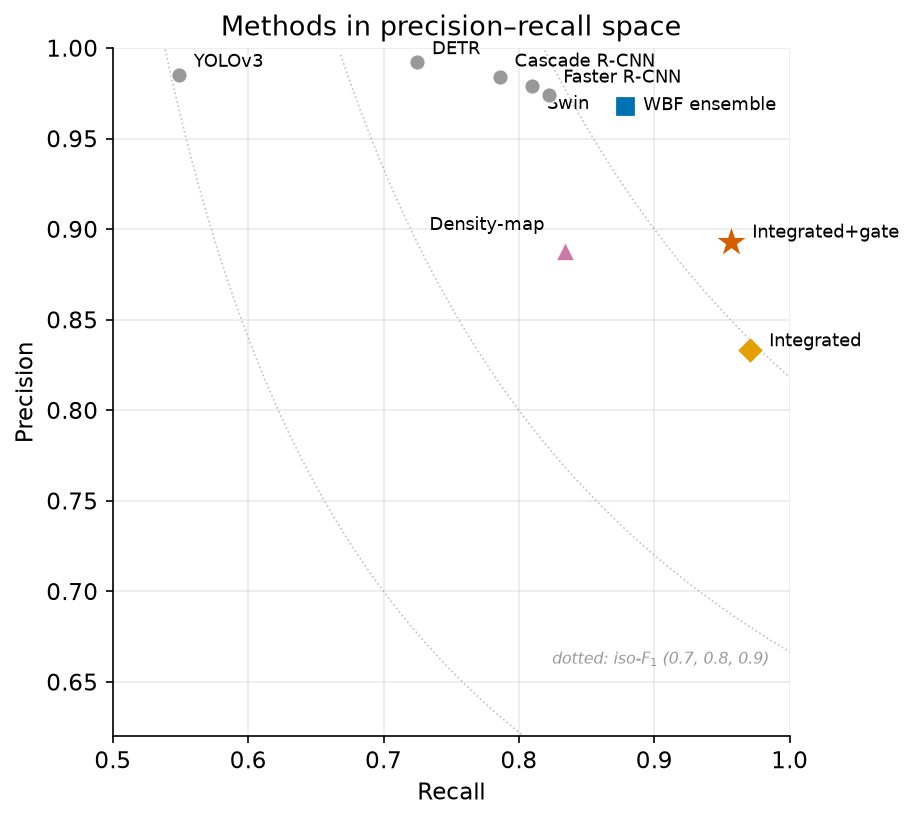
\includegraphics[width=.8\columnwidth]{fig_pr_space.png}
\caption{All methods in precision--recall space, with iso-$F_1$ contours. Individual detectors are high-precision/low-recall; the integrated method with the appearance gate reaches the best-$F_1$ region at high recall.}\label{fig:pr_space}
\end{figure}

For reference, under the recall-only protocol of the conference version (a crown counts as detected if any prediction center falls within it), the ensemble reaches 91.2\% (12{,}353/13{,}552) and the integrated method 96.0\% (13{,}012/13{,}552). We regard the one-to-one metrics as primary because the recall-only protocol does not penalize false positives.

\subsection{Recovery Beyond the Deep-Ensemble Ceiling}

The central question is whether the traditional step adds detections the deep ensemble fundamentally cannot produce, rather than detections a lower threshold would also yield. We take the union of all six detectors' boxes at their \emph{most permissive} score thresholds --- the theoretical ceiling of the deep-learning stack --- and measure ground-truth coverage (Fig.~\ref{fig:workflow_traditional}). This union reaches 94.2\% of trees; the WBF ensemble 92.5\%; the best single detector at most 86.9\%. The integrated method reaches 97.5\%. The traditional step therefore recovers a net 448 crowns (3.3\%) that \emph{no} detector proposes at \emph{any} confidence. The common objection ``lower the detector threshold'' is thus insufficient: every detector is already at its floor.

\paragraph{Why the detectors miss these crowns.} Fig.~\ref{fig:beyond} compares the beyond-ceiling crowns to the detected population. Beyond-ceiling crowns have a median area of 788\,px$^2$ versus 1924\,px$^2$ for detected crowns ($2.44\times$ smaller; 82\% below the 25th percentile of detected-crown area) and are brighter, less saturated, and lower in excess-green --- small and spectrally faint --- yet retain higher local texture contrast. Appearance-trained detectors are least confident on small faint crowns and drop them below any usable threshold, whereas a texture/extremum operator, not relying on learned appearance priors, still fires. Fig.~\ref{fig:qual} shows these recoveries on example images: the recovered crowns (red) are consistently the small, faint ones the detector (blue) missed.

\begin{figure}[htbp]
\centering
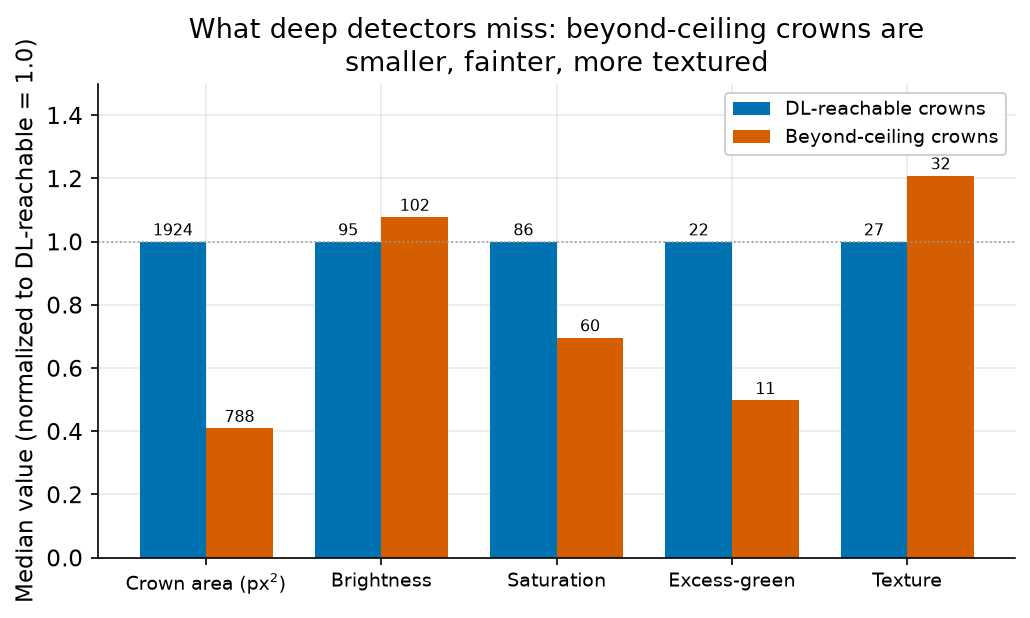
\includegraphics[width=.85\columnwidth]{fig_beyond_features.png}
\caption{Median properties of ground-truth crowns reachable by the deep-detector union versus those recovered only beyond that ceiling. Recovered crowns are smaller, fainter (lower saturation and excess-green), and more textured.}\label{fig:beyond}
\end{figure}

\begin{figure*}[htbp]
\centering
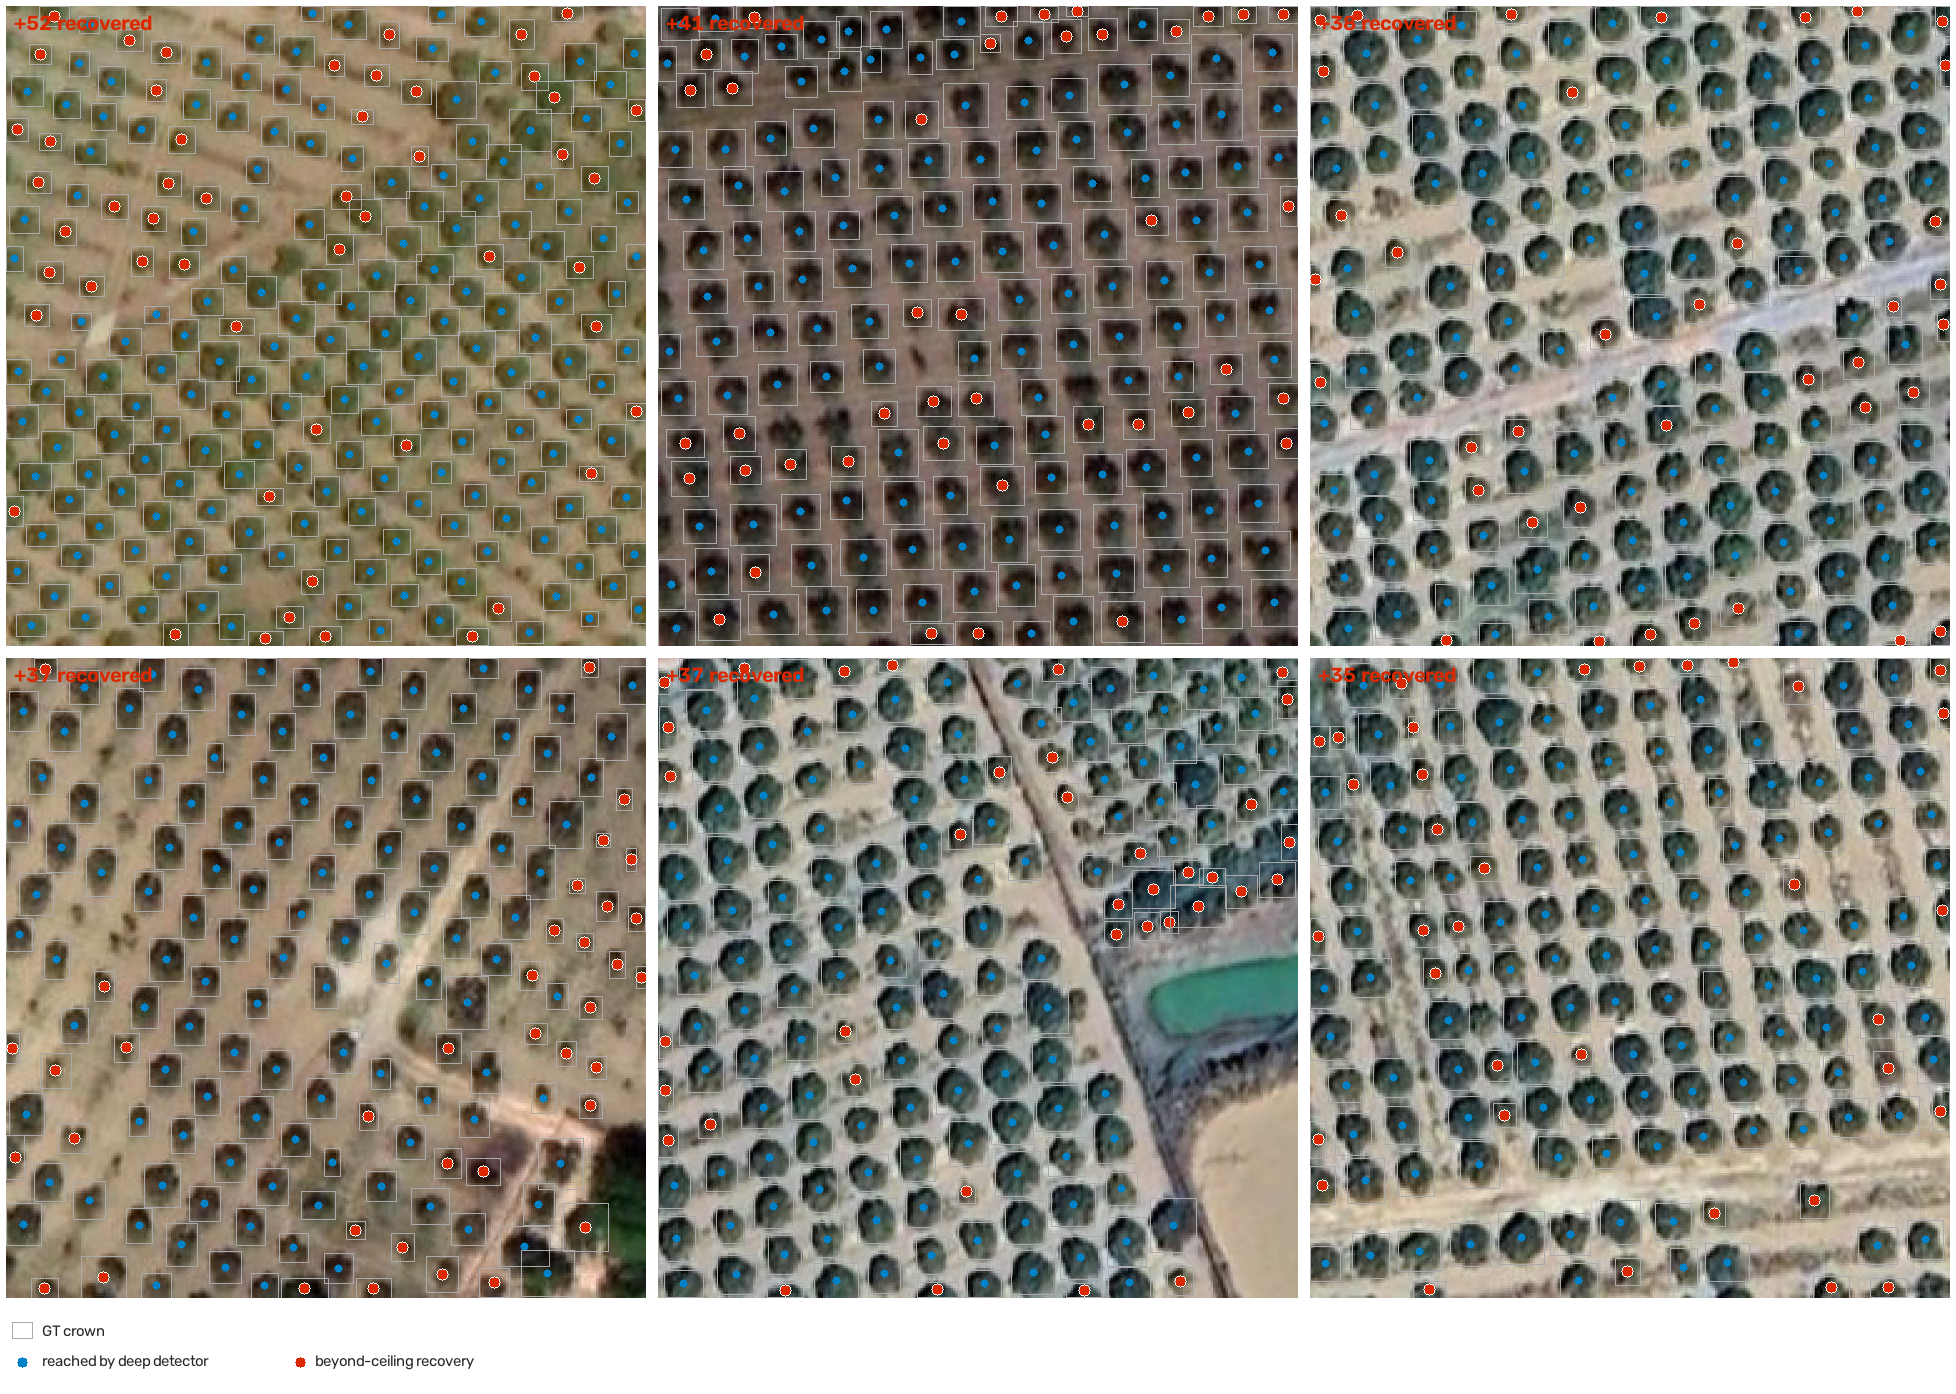
\includegraphics[width=.98\textwidth]{qual_vhrtrees.png}
\caption{Qualitative results on VHRTrees. Grey boxes are ground-truth crowns; blue dots are crowns reached by the deep-learning stack; red dots are beyond-ceiling recoveries --- crowns the detectors missed that the traditional step recovered. Recoveries concentrate on small and edge crowns.}\label{fig:qual}
\end{figure*}

\subsection{The Precision Cost and the Appearance Gate}

Recovering faint crowns also introduces false positives: traditional-only detections fire on grass, bare soil, and rooftops, so the integrated method trades precision (0.833) for recall (0.971) relative to the ensemble. Of its 2{,}647 false positives, 85\% are traditional-only points far from any reliable detector box. We therefore add a lightweight appearance gate: for each traditional-only candidate we classify a crown-sized crop as tree vs.\ non-tree from brightness, chromaticity, and texture features (a logistic classifier), keeping detections near a reliable box unconditionally. Trained and evaluated on image-disjoint halves of the test set, the gate has a tunable threshold that trades precision against retention of the beyond-ceiling recoveries (Fig.~\ref{fig:gate}). Because those recoveries are the paper's central finding, we adopt a \emph{recovery-preserving} operating point that keeps 94\% of them while improving precision to 0.893 (recall 0.957, $F_1$ 0.924), already exceeding the ensemble's 0.921 at a recall it cannot reach. A more aggressive threshold attains $F_1$ 0.934 (precision 0.962, recall 0.908) but retains only 38\% of the recoveries; we therefore do not adopt it as primary.

\begin{figure}[htbp]
\centering
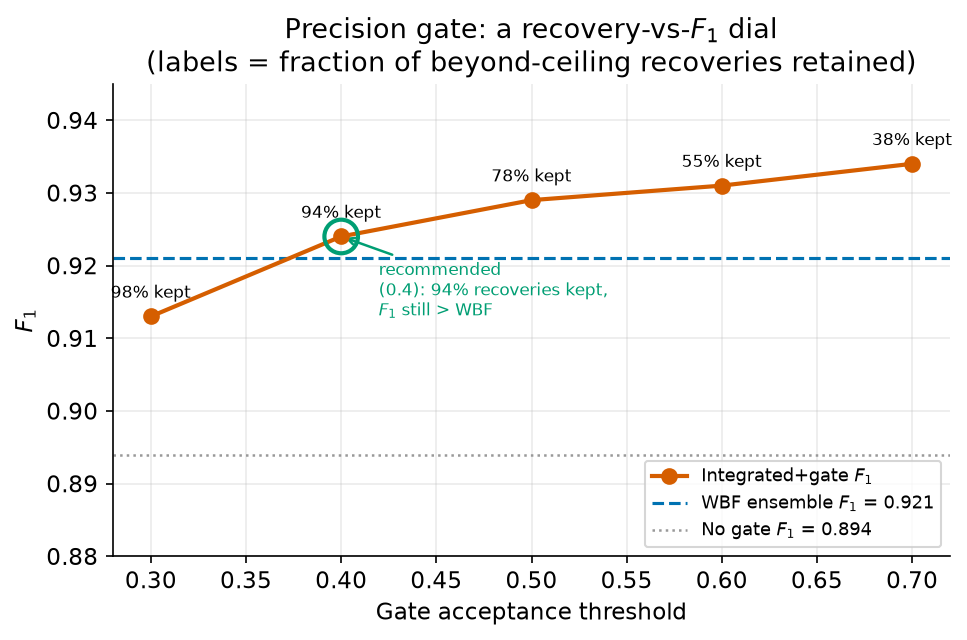
\includegraphics[width=.75\columnwidth]{fig_gate_dial.png}
\caption{The appearance gate as a recovery-vs-$F_1$ dial. Labels give the fraction of beyond-ceiling recoveries retained at each threshold. The recovery-preserving point (0.4) keeps 94\% of recoveries while still exceeding the WBF ensemble's $F_1$.}\label{fig:gate}
\end{figure}

\subsection{Within-dataset Generalization}
Using scene prefixes in the test filenames as an acquisition/region proxy, we test whether the findings hold on unseen scenes (Fig.~\ref{fig:scene}). The beyond-ceiling recovery is a \emph{targeted} benefit: its per-scene gain correlates $-0.98$ with detector strength, i.e.\ it helps most where the detectors are weakest (+10 to +18 pp on low-coverage scenes) and is neutral where they saturate. In a leave-one-scene-group-out test, the appearance gate improves $F_1$ on 7 of 9 held-out scene groups (mean $+0.008$), so it is not merely fit to the test set.

\begin{figure}[htbp]
\centering
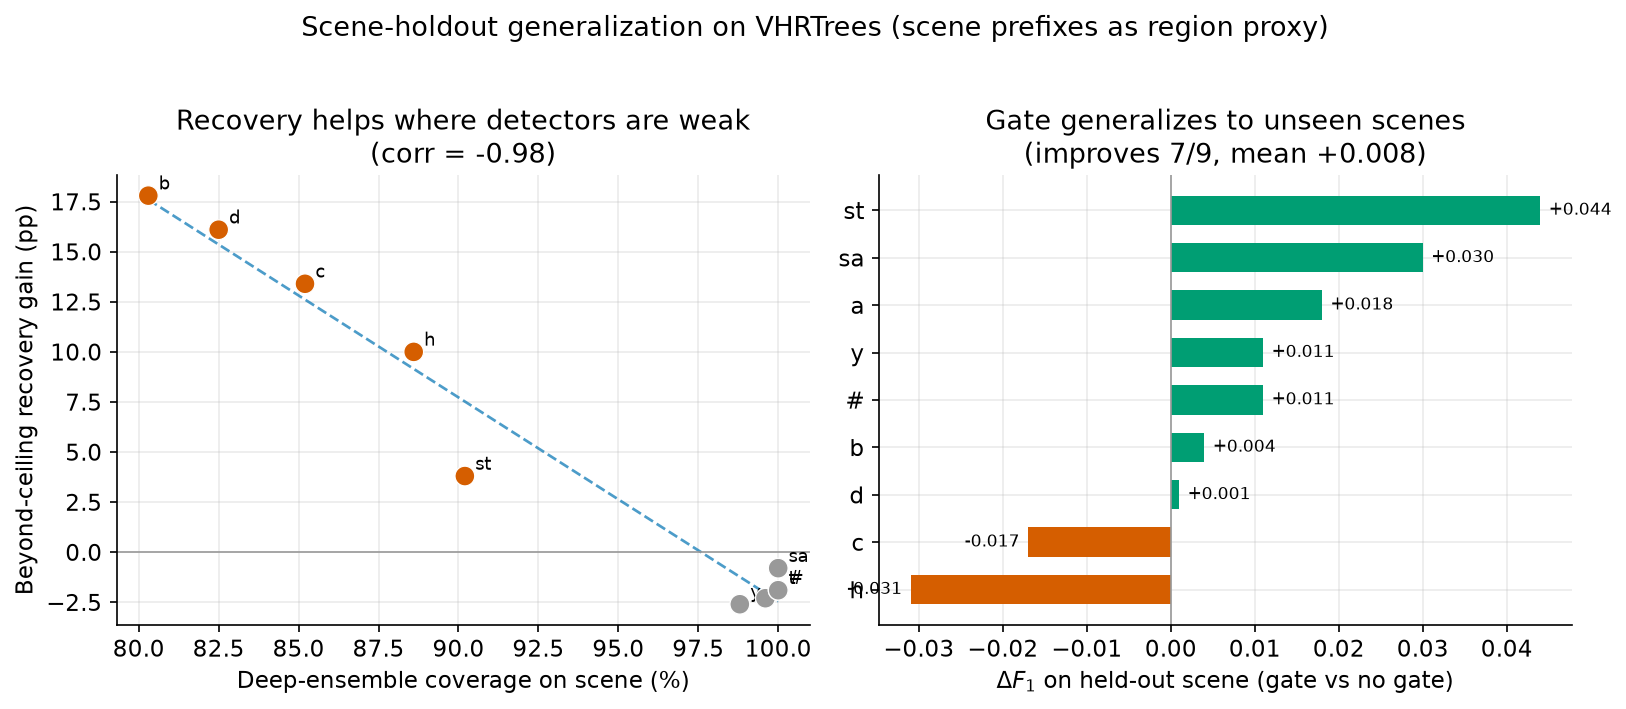
\includegraphics[width=.98\columnwidth]{fig_scene_holdout.png}
\caption{Scene-holdout generalization. Left: per-scene recovery gain versus deep-ensemble coverage (correlation $-0.98$); recovery helps where detectors are weak. Right: gate $\Delta F_1$ on held-out scene groups.}\label{fig:scene}
\end{figure}

\subsection{Cross-dataset Generalization: NEON}
To test whether the mechanism generalizes beyond VHRTrees, we evaluate on the NeonTreeEvaluation benchmark (109 annotated RGB tiles, 3{,}762 trees, US NEON forest sites; airborne imagery, a different biome and sensor). As the deep detector we use DeepForest, the field-standard NEON-trained tree detector, so it is competent on its home data and there is no domain-shift confound. DeepForest reaches 78.4\% of trees; adding the traditional operator raises union coverage to 94.2\%, and the recovered crowns are again the small ones --- median area $1.91\times$ smaller than DeepForest-reached crowns (Fig.~\ref{fig:neon}). The small-crown recovery mechanism therefore replicates across continent, sensor, and detector. We are explicit about the boundary: the traditional pipeline's parameters were tuned on VHRTrees, and its standalone precision on NEON is low (0.25; it over-fires on dense conifer canopy). Thus the \emph{phenomenon} generalizes, while the turnkey pipeline requires per-biome recalibration.

\begin{figure*}[htbp]
\centering
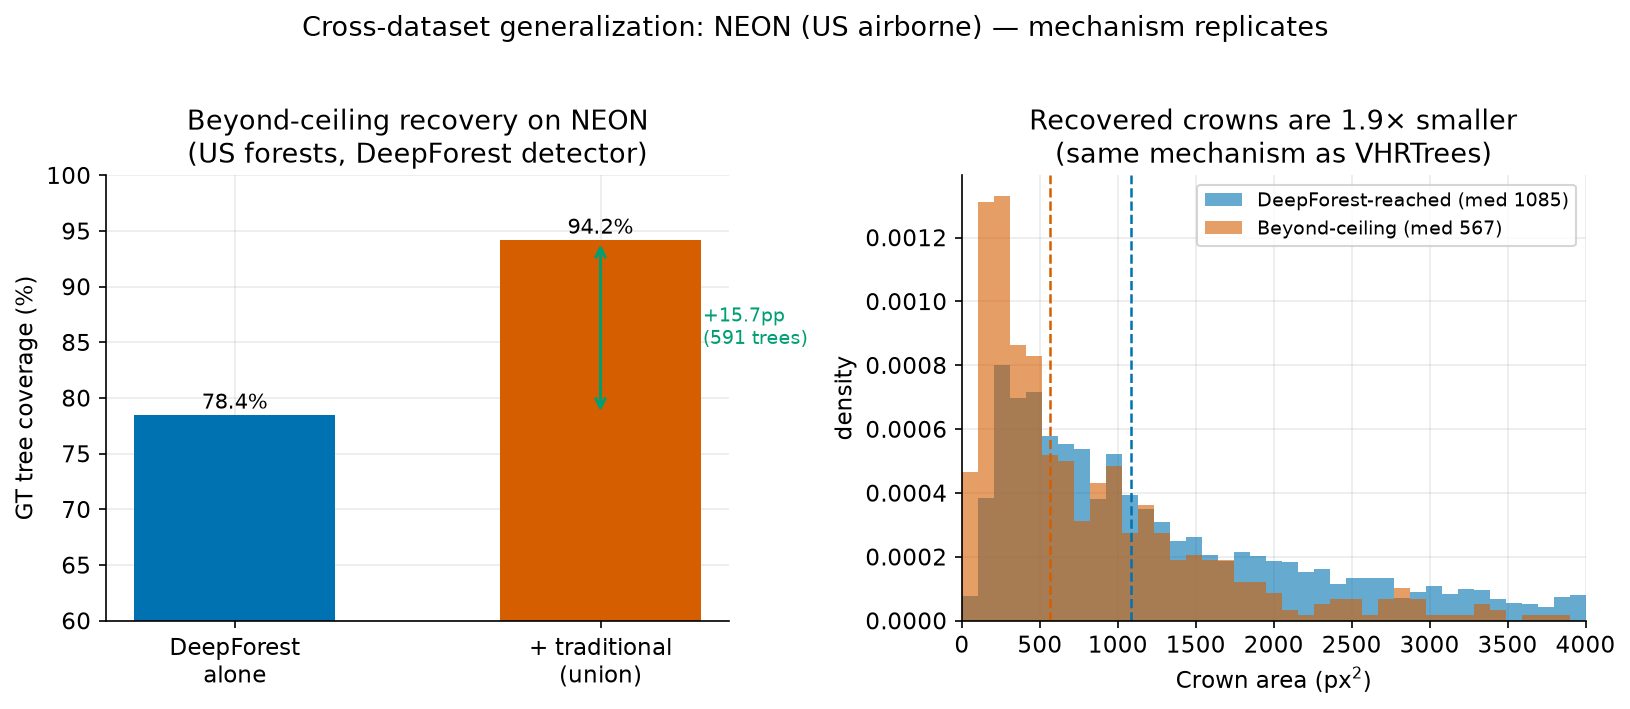
\includegraphics[width=.98\textwidth]{fig_neon_cross.png}
\caption{Cross-dataset test on NEON (US airborne forests) with DeepForest as the detector. Left: coverage; the traditional operator recovers crowns beyond DeepForest. Right: recovered crowns are $1.91\times$ smaller than DeepForest-reached crowns --- the same mechanism observed on VHRTrees.}\label{fig:neon}
\end{figure*}

\subsection{Modern Baseline: Density-map Counter}\label{sec:density}
Because density-map regression is the modern approach for dense small-tree detection, we train a CSRNet-style density counter on the VHRTrees training split and evaluate it identically (Table~\ref{tab:results}). It is a strong \emph{counter} (test count MAE 4.63 trees/image) but a weaker \emph{detector}: its best detection $F_1$ is 0.860 (peak-decode thresholds tuned for best $F_1$), below both the ensemble and the integrated method. Density regression blurs instances into a continuous surface to count robustly; recovering discrete, well-localized centers from that surface is lossy, especially where crowns merge. This supports the detection-centric design for individual-tree localization, while acknowledging density methods are competitive when the goal is counting.

\subsection{Discussion}
Our results show that a traditional operator contributes detections a strong deep ensemble cannot, that these are specifically the small, faint crowns, and that a simple appearance gate converts the resulting recall gain into an operating point that dominates the ensemble. The complementarity is a targeted safety-net: most valuable where deep detection is weakest, which is precisely where a practitioner needs it. Beyond detection, the traditional segmentation can supply canopy information and can serve as an automatic, partial labeler for unlabeled imagery, on which the deep models can then be trained and the rule-based step reapplied to refine results.

\subsection{Limitations}
Three limitations bound our claims. First, while the mechanism replicates on NEON, the specific magnitude (3.3 pp) and the appearance-gate coefficients are dataset-dependent, and the traditional pipeline requires per-biome recalibration (its untuned NEON precision is 0.25). Second, ``beyond-ceiling'' is defined relative to these six detectors (or DeepForest on NEON); a detector trained specifically for tiny crowns could shrink the gap, so the finding characterizes the complementarity of current strong detectors rather than a permanent limit. Third, the appearance gate is supervised; for unlabeled imagery it must be trained once on a labeled subset, which the image-disjoint evaluation here is designed to estimate.

\section{Conclusion}
We combined traditional and deep learning methods for tree crown detection through a rule-based integration, and --- rather than reporting a single recall figure --- measured and explained the complementarity between them. A traditional operator recovers 3.3\% of trees beyond the ceiling of a six-model deep ensemble; these are systematically small, faint crowns; an appearance gate makes the integrated detector dominate the ensemble on the precision--recall frontier; and the recovery mechanism replicates on an independent US airborne benchmark with the field-standard detector. Traditional methods thus retain a specific, quantifiable value in the deep-learning era: recovering the small crowns that appearance-trained detectors systematically miss.

\section*{Declarations}
\subsection*{Funding}
This study is supported by TUBITAK Project No.\ 221N393 and Project ForestMap. Project ForestMap is supported under the umbrella of ERANET Cofund ForestValue by the Swedish Governmental Agency for Innovation Systems, Swedish Energy Agency, The Swedish Research Council for Environment, Agricultural Sciences and Spatial Planning, Academy of Finland, and TUBITAK. ForestValue has received funding from the European Union's Horizon 2020 research and innovation programme under grant agreement No.\ 773324 and from TUBITAK Project No.\ 221N393.

\subsection*{Code and Data Availability}
The VHRTrees data are available at \textit{RSandAI/VHRTrees} \cite{10.3389/ffgc.2024.1495544}. The NEON benchmark is the public NeonTreeEvaluation dataset. Source code, the evaluation and integration modules, trained models, and the scripts that reproduce every number and figure in this paper are available at \url{https://github.com/ozan956/Tree-Crown-Detection}.

%Bibliography
\bibliographystyle{unsrt}
\bibliography{references}

\end{document}
